\documentclass[11pt,a4paper]{article}
\usepackage[margin=2.2cm]{geometry}
\usepackage[T1]{fontenc}
\usepackage{lmodern,microtype}
\usepackage{graphicx,booktabs,tabularx,float,caption,xcolor,enumitem,amsmath,array,multirow}
\usepackage[hidelinks]{hyperref}
\graphicspath{{../figures/}{../../results/plots/}}
\captionsetup{font=small,labelfont=bf}
\setlist{itemsep=2pt,topsep=4pt}
\newcolumntype{R}{>{\raggedleft\arraybackslash}X}

\title{\textbf{Processing and Visualising Large DEMs on a Laptop}\\[4pt]
\large Progress Report: Data Preparation and Baseline Benchmarks of Standard Terrain Tools}
\author{Team GeoGuessers \quad|\quad Spatial Informatics\\[4pt]
Swayam Goyal (2024111012) \quad Siddharth Choudhary (2024111021)\\
Yakkala Viswanadha Kartikeya (2024111033)}
\date{}

\begin{document}
\maketitle

\begin{abstract}
\noindent
We investigate how far large, high-resolution Digital Elevation Models (DEMs) can be processed and visualised on a
single laptop, and where the actual bottleneck lies. On one Himalayan study area (Uttarakhand, $\sim$100\,km
$\times$ 100\,km) we prepared real DEMs at 90, 30, 8 and 2\,m and synthetic 2\,m and 1\,m grids (up to 10.8 billion
cells, 43\,GB as float32, 2.7$\times$ the laptop's RAM). With a purpose-built benchmark harness that measures exact
per-process time, memory, CPU and I/O under controlled cold- and warm-cache conditions, we ran 832 measured runs of
GDAL's \texttt{gdaldem} (10 operator/method configurations), seven storage layouts, and QGIS rendering. Three findings
stand out. (1) \texttt{gdaldem} never runs out of memory: it streams the grid and peaks at 0.83\,GB even at 1\,m; it
only slows down linearly, at 20--25\,ns per cell (3.5\,min for one slope pass at 1\,m). (2) The bottleneck is
single-threaded computation ($\sim$73\% of run time, 1 of 22 threads used), not disk (14\%) or memory; the file-cache
state changes run time by $\le$2\%. (3) For display, the bottleneck is reading full-resolution data: without a
pyramid, a whole-area QGIS redraw takes 32\,s at 1\,m, with one it takes 0.09\,s at every resolution. These results
motivate the next phase: a tiled, parallel CPU/GPU engine and on-demand computation from pyramid levels.
\end{abstract}

\section{Objectives}
Following our discussion, the project is approached as a systems study: given a very large, high-resolution DEM and
limited hardware, determine how to process and visualise only the data currently required, using multi-resolution
(pyramid) representations, on-the-fly computation and appropriate CPU/GPU processing, while identifying the actual
bottleneck rather than assuming one. Our literature review identified two gaps that this project addresses:
\begin{itemize}
  \item[\textbf{G1}] No study reports where standard GDAL/QGIS terrain tools stop being practical on a single laptop,
  separated into stages (disk read, computation, write, display).
  \item[\textbf{G2}] No study computes terrain derivatives on demand from pyramid levels, or measures the error of
  coarse-level slope against the time it saves.
\end{itemize}
This report covers the work towards G1: data preparation, the benchmark methodology, and the baseline measurements.

\section{Data}
All experiments use one study area, so that grid size is the only variable that changes (Figure~\ref{fig:area},
Table~\ref{tab:data}). The area is HMA tile-571 in the Garhwal Himalaya (Nanda Devi region), with elevations from
670\,m to 7{,}790\,m. All grids were reprojected to WGS\,84 / UTM 44N (EPSG:32644) on one aligned grid and stored as
Cloud-Optimized GeoTIFFs (512-pixel tiles, ZSTD compression, internal overviews forming the pyramid).

\begin{figure}[H]
\centering
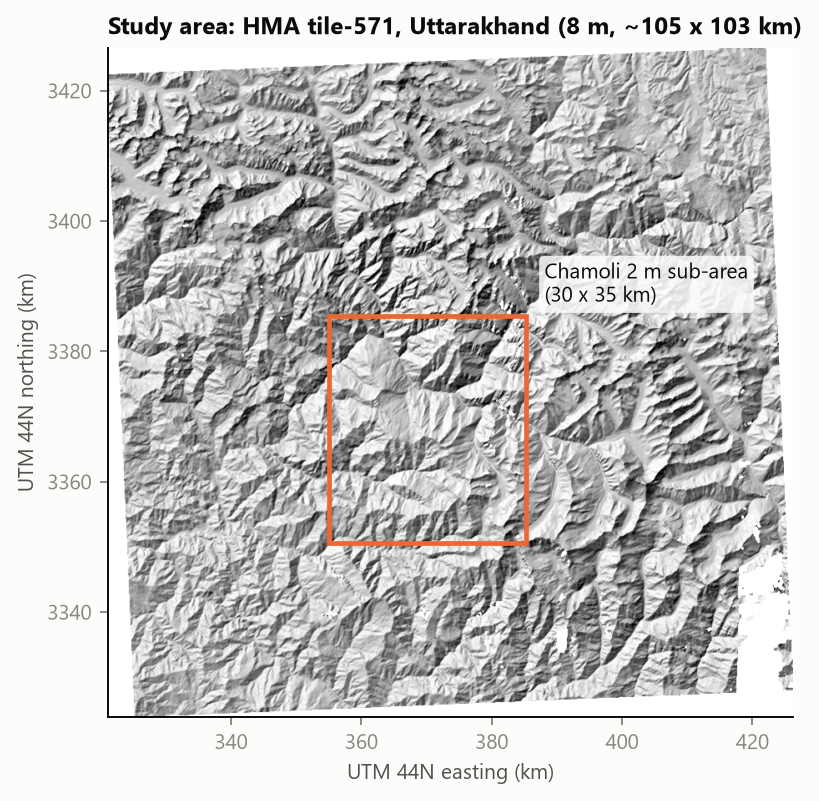
\includegraphics[width=0.55\linewidth]{study_area.png}
\caption{Study area (shaded relief of the 8\,m DEM) and the Chamoli sub-area covered by the real 2\,m DEM.}
\label{fig:area}
\end{figure}

\begin{table}[H]
\centering\small
\caption{Resolution ladder. Real grids are used for timing and accuracy; synthetic grids only for timing.}
\label{tab:data}
\begin{tabularx}{\linewidth}{lllrX}
\toprule
Res. & Source & Type & Cells & Role \\
\midrule
90\,m & Copernicus GLO-90 (OpenTopography) & real & 1.3\,M & coarsest level \\
30\,m & Copernicus GLO-30 \cite{cop30} & real & 12\,M & baseline level \\
8\,m & NASA High Mountain Asia 8\,m mosaic \cite{hma8} & real & 169\,M & finest real level, whole area \\
2\,m & Chamoli 2\,m composite \cite{chamoli} & real & 264\,M & accuracy truth (sub-area) \\
2\,m & cubic upsample of the 8\,m tile & synthetic & 2.7\,B & timing only \\
1\,m & cubic upsample of the 8\,m tile & synthetic & 10.8\,B & timing only; 43\,GB $>$ 16\,GB RAM \\
\bottomrule
\end{tabularx}
\end{table}

\paragraph{Data checks.} All downloads were checksum-verified. The 2\,m and 8\,m DEMs agree well where they overlap
(2\,m averaged to 8\,m minus the 8\,m DEM: median $-0.7$\,m, NMAD 5.1\,m over 14 million cells). The 8\,m DEM sits
24.5\,m below Copernicus (ellipsoidal vs geoid heights), which does not affect slope, aspect or hillshade. Since no
free 1\,m DEM exists for this region, we tested how reliable synthetic grids are: on a 16-million-cell crop, an 8\,m
grid rebuilt from 16\,m gave the same \texttt{gdaldem} run time as the real one (0.87--0.90\,s) but 2.3--3.0$^\circ$
slope RMSE. Synthetic grids are therefore used for timing only, with cubic resampling (nearest-neighbour data
compresses 26\% better than real terrain and would distort read times).

\section{Benchmark methodology}
\paragraph{Machine.} Intel Core Ultra 9 185H (6 performance, 8 efficiency and 2 low-power cores; 22 threads), 16\,GB
RAM, NVMe SSD ($\sim$2\,GB/s reads), NVIDIA RTX 4060 Laptop GPU (8\,GB, not used by these tools), Windows 11,
GDAL 3.13.3, QGIS 3.44.14.

\paragraph{Harness.} Each measurement runs one tool as a separate process. For every run we record wall time and,
read exactly from the finished process, its peak memory (peak working set), CPU time and bytes read/written, plus
the bytes physically read from disk. One row per run is stored with the dataset, operator, method, cache state and
the code version. Sweeps are resumable.

\paragraph{Protocol.}
\begin{itemize}
  \item \textbf{Cold cache:} the Windows file cache (standby list) is emptied before each cold run (Sysinternals
  RAMMap); we verified that the whole file is then read from disk again. \textbf{Warm cache:} immediate repeat.
  \item \textbf{Repeats:} real grids: 5 cold runs and 1 warm-up + 5 warm runs; synthetic 2\,m/1\,m: 3 cold + 1 warm.
  Medians are reported.
  \item \textbf{Core pinning:} \texttt{gdaldem} measured 1.7$\times$ slower on an efficiency core and up to
  2.7$\times$ on a low-power core, and Windows can move a process between them mid-run (one unpinned run took
  108.9\,s instead of 56\,s). All tools are pinned to the performance cores, i.e.\ measured at their best.
  \item \textbf{Background activity:} Windows Defender scanning our 10--40\,GB temporary outputs held disk space and
  slowed following runs by 25--35\%. Only the two scratch folders were excluded from scanning, and the harness waits
  until deleted outputs are released before the next run. All final numbers were re-run under these conditions.
  \item \textbf{Stage split:} two reference runs per grid, a pure read + decompress and a copy to an uncompressed
  GeoTIFF (the same read and same-size write as \texttt{gdaldem}), give write $\approx$ copy $-$ read and
  compute $\approx$ \texttt{gdaldem} $-$ copy.
\end{itemize}

\paragraph{Experiments.} \textbf{E1:} \texttt{gdaldem} slope, aspect, hillshade (Horn and Zevenbergen--Thorne
\cite{horn,zt}), TRI (Riley, Wilson), TPI and roughness on all six grids, cold and warm (560 runs; slope and
hillshade only at 1\,m). \textbf{E2:} seven storage layouts (strips vs tiles, 256 vs 512 tiles, none/LZW/DEFLATE/ZSTD)
of the 8\,m and 2\,m grids: write, read and slope (224 runs). \textbf{QGIS display:} open a layer and render one
1920$\times$1080 view, whole area or zoomed in, with or without the pyramid (48 runs).

\section{Results}
\subsection{E1: \texttt{gdaldem} across grid sizes}

\begin{table}[H]
\centering\small
\caption{\texttt{gdaldem} (Horn) by grid size. Medians; ns/cell for slope, warm cache.}
\label{tab:e1}
\begin{tabularx}{\linewidth}{lRRRRRR}
\toprule
Grid & Cells & Slope cold & Slope warm & Hillshade & ns/cell & Peak memory \\
\midrule
90\,m & 1.3\,M & 0.08\,s & 0.07\,s & 0.06\,s & (start-up) & 41\,MB \\
30\,m & 12\,M & 0.29\,s & 0.28\,s & 0.13\,s & 23.1 & 91\,MB \\
8\,m & 169\,M & 4.10\,s & 4.02\,s & 2.96\,s & 23.8 & 710\,MB \\
2\,m real & 264\,M & 6.67\,s & 6.63\,s & 4.74\,s & 25.1 & 828\,MB \\
2\,m synthetic & 2.7\,B & 54.2\,s & 53.7\,s & 41.0\,s & 19.9 & 830\,MB \\
1\,m synthetic & 10.8\,B & 208.3\,s & 208.4\,s & 158.9\,s & 19.3 & 832\,MB \\
\bottomrule
\end{tabularx}
\end{table}

\begin{itemize}
  \item \textbf{No memory limit:} \texttt{gdaldem} streams the grid and processes 43\,GB of data with 0.83\,GB.
  \item \textbf{Linear time:} 20--25\,ns per cell once start-up stops mattering; 3.5\,min for slope at 1\,m.
  \item \textbf{Single-threaded:} 0.99 of 22 threads used at every size.
  \item \textbf{Cache does not matter:} cold vs warm differ by $\le$2\%. At 2\,m/1\,m the file exceeds what the
  cache can hold, so even warm runs read 3.6/13.6\,GB from disk and take the same time.
\end{itemize}

\begin{figure}[H]
\centering
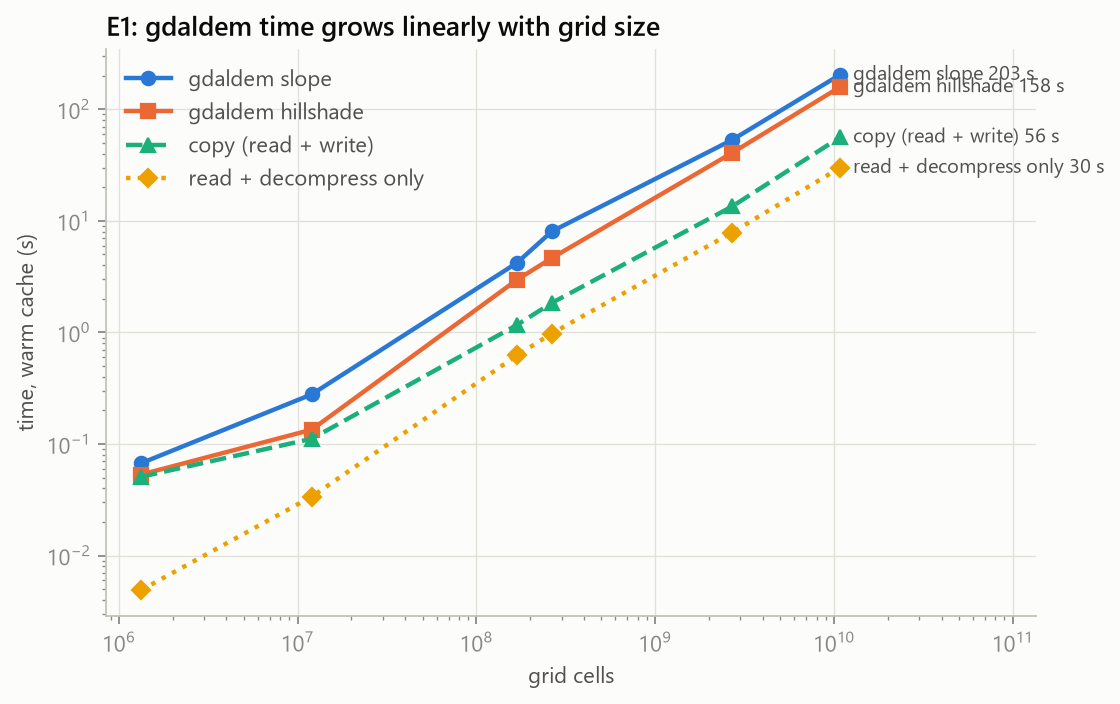
\includegraphics[width=0.49\linewidth]{e1_scaling.png}\hfill
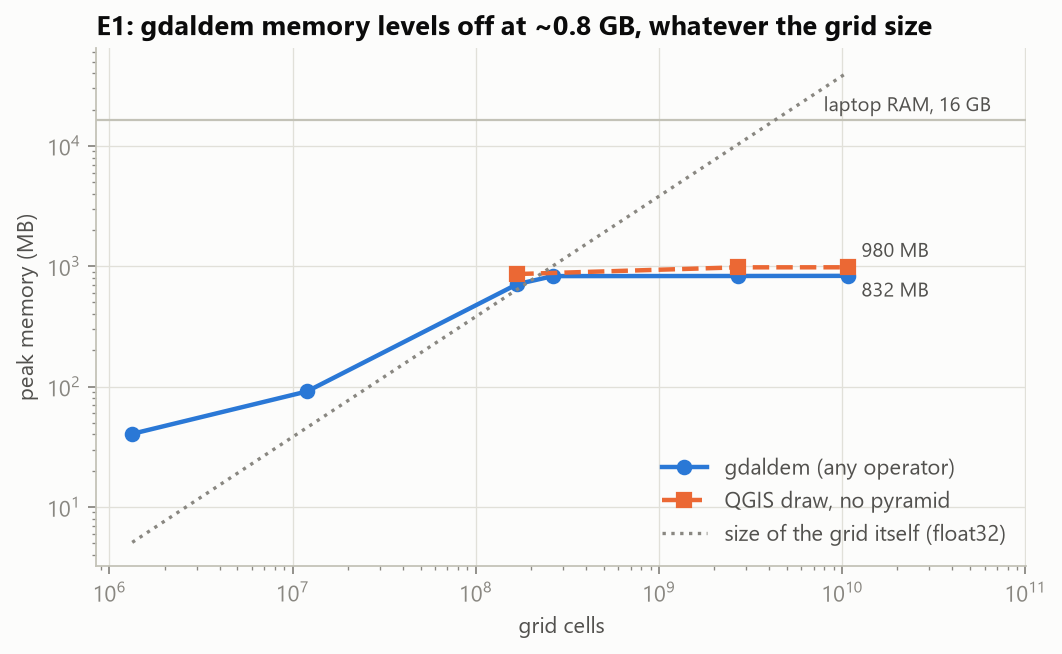
\includegraphics[width=0.49\linewidth]{e1_memory.png}
\caption{Left: run time grows linearly with the number of cells. Right: peak memory levels off at $\sim$0.83\,GB
(GDAL's block cache), far below the size of the grid, which exceeds the 16\,GB RAM at 1\,m.}
\label{fig:e1}
\end{figure}

\begin{figure}[H]
\centering
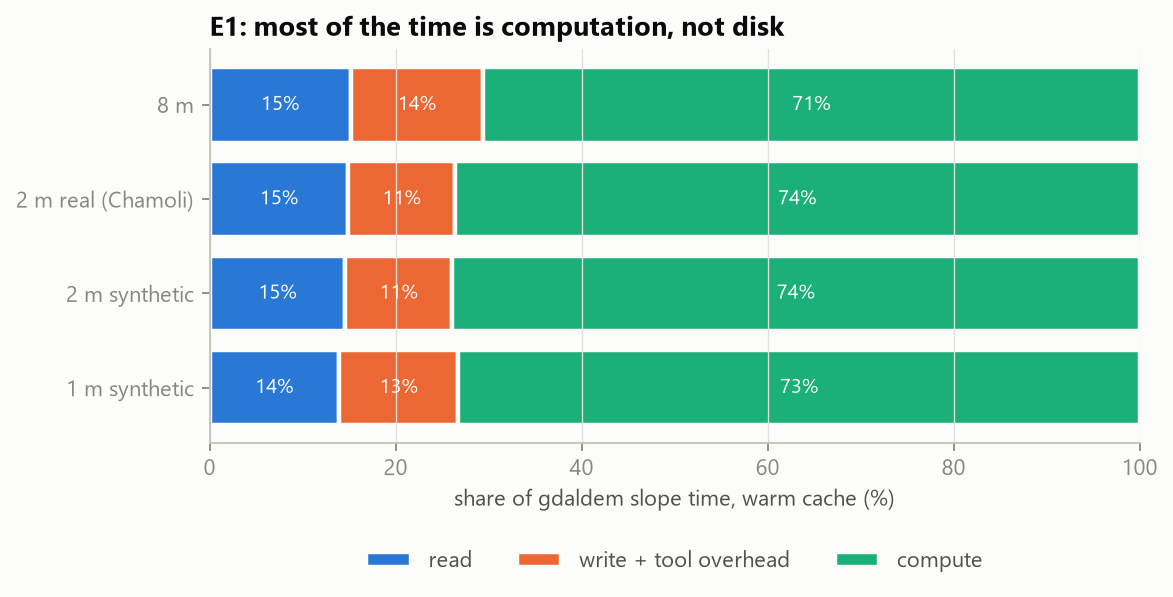
\includegraphics[width=0.49\linewidth]{e1_stages.png}\hfill
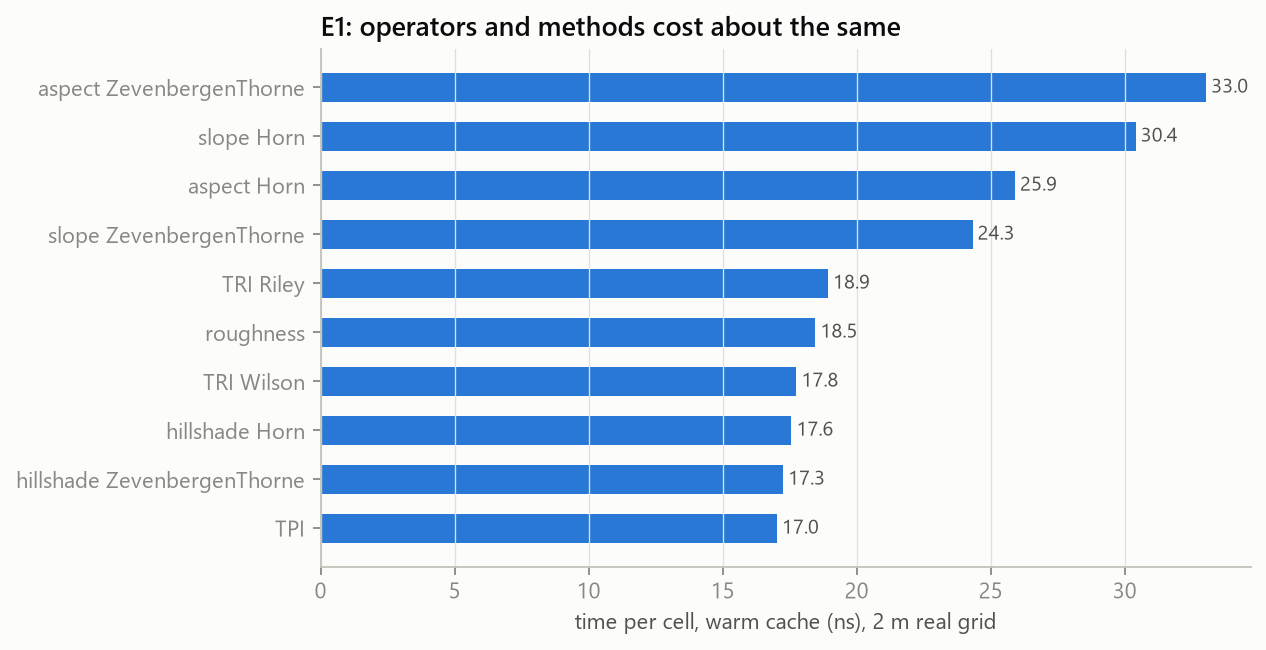
\includegraphics[width=0.49\linewidth]{e1_operators.png}
\caption{Left: share of slope run time per stage; computation is $\sim$73\% at every size. Right: cost per cell of
all ten configurations on the real 2\,m grid.}
\label{fig:e1b}
\end{figure}

All operators cost 17.5--27\,ns per cell; Horn and Zevenbergen--Thorne differ by at most 6\% (slope 4\%, aspect 6\%,
hillshade 0\%). Hillshade is cheaper than slope partly because it writes 1-byte instead of 4-byte output.

\subsection{E2: storage layout}

\begin{table}[H]
\centering\small
\caption{Storage layouts of the 2\,m synthetic grid (2.7 billion cells). Cold-cache medians.}
\label{tab:e2}
\begin{tabularx}{\linewidth}{lRRRR}
\toprule
Layout & File size & Write & Read + decompress & \texttt{gdaldem} slope \\
\midrule
Strips, uncompressed (GDAL default) & 10.3\,GB & 13.9\,s & 4.0\,s & \textbf{47.1\,s} \\
Tiles 256, uncompressed & 10.4\,GB & 13.5\,s & 4.0\,s & 51.8\,s \\
Tiles 512, uncompressed & 10.4\,GB & 13.3\,s & 3.3\,s & 49.1\,s \\
Tiles 512, LZW & 4.8\,GB & 88.9\,s & 20.1\,s & 65.7\,s \\
Tiles 512, DEFLATE & 3.7\,GB & 113.4\,s & 11.4\,s & 57.0\,s \\
\textbf{Tiles 512, ZSTD} (our pyramids) & \textbf{3.6\,GB} & 123.9\,s & \textbf{7.8\,s} & 53.7\,s \\
Tiles 256, ZSTD & 3.7\,GB & 121.0\,s & 8.6\,s & 55.3\,s \\
\bottomrule
\end{tabularx}
\end{table}

Layout changes \texttt{gdaldem} time by up to 40\%, because decompression runs inside the single thread: LZW is 39\%
slower than uncompressed strips, ZSTD only 14\%. ZSTD is the best compressed format (2.9$\times$ smaller than
uncompressed and decoding 2.6$\times$ faster than LZW); LZW, a common default, is worst on speed and nearly worst on
size. Writing compressed files is $\sim$9$\times$ slower, a one-time cost when the pyramid is built. The real 8\,m
grid shows the same pattern (slope 3.42\,s uncompressed, 3.94\,s ZSTD, 4.78\,s LZW).

\begin{figure}[H]
\centering
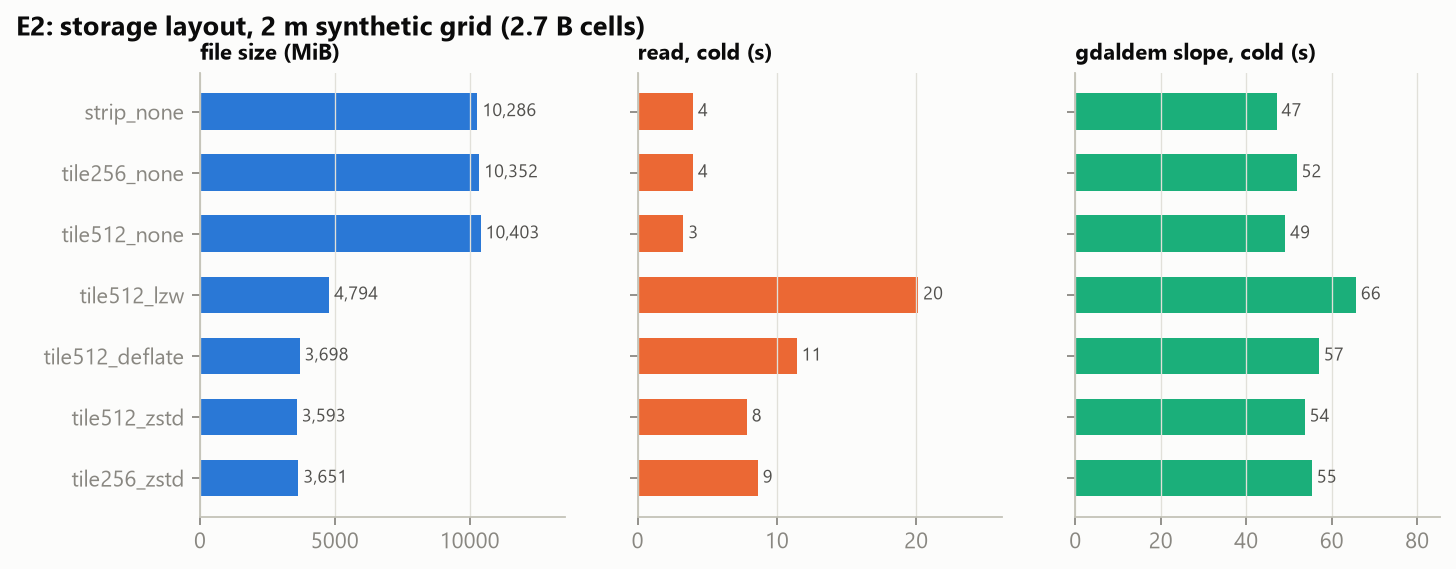
\includegraphics[width=0.9\linewidth]{e2_storage.png}
\caption{E2: file size, read time and \texttt{gdaldem} slope time per storage layout (2\,m synthetic grid).}
\end{figure}

\subsection{QGIS display}

\begin{table}[H]
\centering\small
\caption{QGIS: time to render one 1920$\times$1080 view (cold cache), and peak memory for the whole-area view.}
\label{tab:qgis}
\begin{tabularx}{\linewidth}{lRRRR}
\toprule
Grid & Whole area, pyramid & Whole area, no pyramid & Zoomed in (either) & Peak memory (pyramid / none) \\
\midrule
8\,m & 0.09\,s & 0.79\,s & 0.10\,s & 199 / 862\,MB \\
2\,m synthetic & 0.09\,s & 8.82\,s & 0.10\,s & 200 / 979\,MB \\
1\,m synthetic & 0.09\,s & \textbf{31.9\,s} & 0.11\,s & 200 / 980\,MB \\
\bottomrule
\end{tabularx}
\end{table}

\begin{figure}[H]
\centering
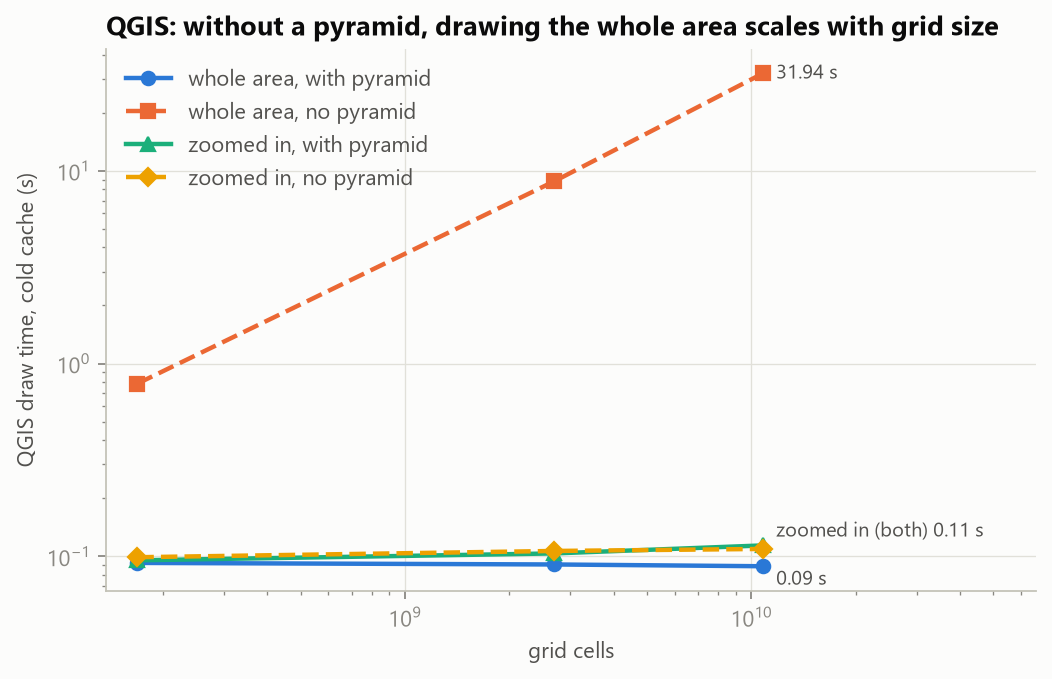
\includegraphics[width=0.62\linewidth]{e1q_render.png}
\caption{Without a pyramid, a whole-area redraw reads the full-resolution grid and grows with its size; with the
pyramid, and for zoomed-in views, the cost stays constant.}
\end{figure}

Opening a layer takes 0.02--0.03\,s in all cases. Only zoomed-out views need the pyramid: a zoomed-in view reads just
its window. Without a pyramid, each whole-area redraw of the 1\,m grid reads the entire 16.6\,GB file
(350$\times$ slower than with the pyramid), which makes interactive use impossible.

\section{Discussion}
\paragraph{Where standard tools stop being practical (G1).} On a 16\,GB laptop with an NVMe SSD the standard tools
do not fail at 1\,m; they stop being practical. Processing is limited by single-threaded computation, with disk
and memory far from their limits. Display is limited by reading full-resolution data when no pyramid is used.

\paragraph{Comparison with the literature and our pilot.} The literature generally reports data movement as the main
limit for large rasters, and our pilot test saw a $\sim$3$\times$ difference between uncached and cached runs at
5\,m. With a verified cold cache and a fast NVMe SSD, we instead find \texttt{gdaldem} to be compute-bound
($\sim$73\%) and the cache state to be irrelevant ($\le$2\%). The pilot timed runs through the QGIS interface on a
different laptop, so its first runs likely included one-off start-up and loading costs. For display, our results
agree with the pyramid-based approaches of Losasso and Hoppe \cite{clipmaps} and Campos et al.\ \cite{campos}.

\paragraph{Implications.} (1) The largest gain for processing should come from parallel computation across the
22 threads; decompression must also be parallel, since reading and decompressing the 1\,m grid alone takes 29\,s on
one thread while the SSD could deliver it in $\sim$8\,s. (2) Computing several derivatives in one pass avoids
re-reading and re-writing the grid ($\sim$27\% of each \texttt{gdaldem} run). (3) On-demand computation is cheap:
slope for one 256$\times$256 tile costs $\sim$1.6\,ms on one thread, so an interactive viewer is limited by reading
the right window at the right pyramid level.

\paragraph{Validity.} Most configurations repeat within 0.2--3.3\% (median spread); medians absorb the few single
slow runs. Runs below $\sim$10 million cells are dominated by program start-up and are not used for per-cell claims.
Synthetic grids are used only for timing. Earlier, disturbed attempts (before pinning and before handling background
scanning) are kept as evidence.

\section{Next steps}
\begin{enumerate}
  \item \textbf{Our engine (E3, E4):} tiled processing with overlapping borders (halos), NumPy reference, Numba
  parallel CPU and CuPy GPU kernels for the same six operators, computing several derivatives in one pass; validated
  against \texttt{gdaldem}; measured against the baseline above, including CPU--GPU transfer times.
  \item \textbf{Pyramid on demand (E5, gap G2):} compute slope directly from each pyramid level and measure its error
  against the real 2\,m slope, together with the time saved, split by slope class.
  \item \textbf{Interactive viewer (E6):} a tile server computing slope/aspect/hillshade tiles on the fly for QGIS
  and a Cesium globe; tile latency for precomputed vs on-the-fly CPU vs GPU.
  \item \textbf{Stretch:} viewshed (R3 vs XDraw vs \texttt{gdal\_viewshed}) and terrain distance (Dijkstra vs A*).
\end{enumerate}

\begin{thebibliography}{9}\small
\bibitem{cop30} European Space Agency (2021). Copernicus Global Digital Elevation Model (GLO-30). Distributed by
OpenTopography. doi:10.5069/G9028PQB.
\bibitem{hma8} Shean, D. (2017). High Mountain Asia 8-meter DEM Mosaics Derived from Optical Imagery, Version 1.
NASA NSIDC DAAC. doi:10.5067/KXOVQ9L172S2.
\bibitem{chamoli} Bhushan, S., \& Shean, D. (2021). Chamoli Disaster Pre-event 2-m DEM Composite: September 2015.
Zenodo. doi:10.5281/zenodo.4554647.
\bibitem{horn} Horn, B.\,K.\,P. (1981). Hill shading and the reflectance map. \emph{Proceedings of the IEEE},
69(1), 14--47.
\bibitem{zt} Zevenbergen, L.\,W., \& Thorne, C.\,R. (1987). Quantitative analysis of land surface topography.
\emph{Earth Surface Processes and Landforms}, 12(1), 47--56.
\bibitem{clipmaps} Losasso, F., \& Hoppe, H. (2004). Geometry clipmaps: Terrain rendering using nested regular
grids. \emph{ACM Transactions on Graphics}, 23(3), 769--776.
\bibitem{campos} Campos, R., et al.\ (2020). 3D simplification methods and large scale terrain tiling.
\emph{Remote Sensing}, 12(3), 437.
\end{thebibliography}

\end{document}
